\begin{titlepage}

  \setlength{\parindent}{0pt}
  \thispagestyle{empty}

  \begin{center}
  
\includegraphics[height=3cm]{content/logo}
  \end{center}

  \bigskip

  \begin{center}
  \fontsize{14pt}{16pt}\selectfont
  \textbf{THÈSE DE DOCTORAT DE L'UNIVERSITÉ DE LYON}\\

  \bigskip

  \fontsize{12pt}{14pt}\selectfont
  \textbf{Opérée au sein de}\\ \medskip
  l'Université Claude Bernard Lyon 1

  \textbf{École doctorale}\\ \medskip
  Neurosciences et Cognition (ED476)

  \textbf{Spécialité de doctorat}\\ \medskip
  Neurosciences

  Soutenue publiquement le 8 décembre 2017 par\\ \medskip
  \fontsize{14pt}{16pt}\selectfont
  \textbf{\thesisName}

  \rule{\textwidth}{0.5pt}

  \fontsize{16pt}{20pt}\selectfont
  \textbf{FRÉQUENCE ET CONTENU DU RAPPORT DE RÊVE:\\ \medskip
  Approches Comportementales et Neurophysiologiques.}
  \rule{\textwidth}{0.5pt}

  \end{center}

  \fontsize{12pt}{14pt}\selectfont
  \textbf{Devant le jury composé de:}

  \newcommand\textline[4][t]{%
      \par\noindent\parbox[#1]{.333\textwidth}{\raggedright#2}%
      \parbox[#1]{.333\textwidth}{\centering#3}%
      \parbox[#1]{.333\textwidth}{\raggedleft#4}\par
  }

  \textline[t]{Pr. Sophie SCHARTZ}{Université de Genève}{Rapporteure}
  \textline[t]{Pr. Michael SCHREDL}{CIMH}{Rapporteur}
  \textline[t]{Pr. Yves ROSSETTI}{Université de Lyon}{Examinateur}
  \textline[t]{Pr. Perrine RUBY }{Université de Lyon}{Directrice de thèse}

\end{titlepage}

\cleardoublepage
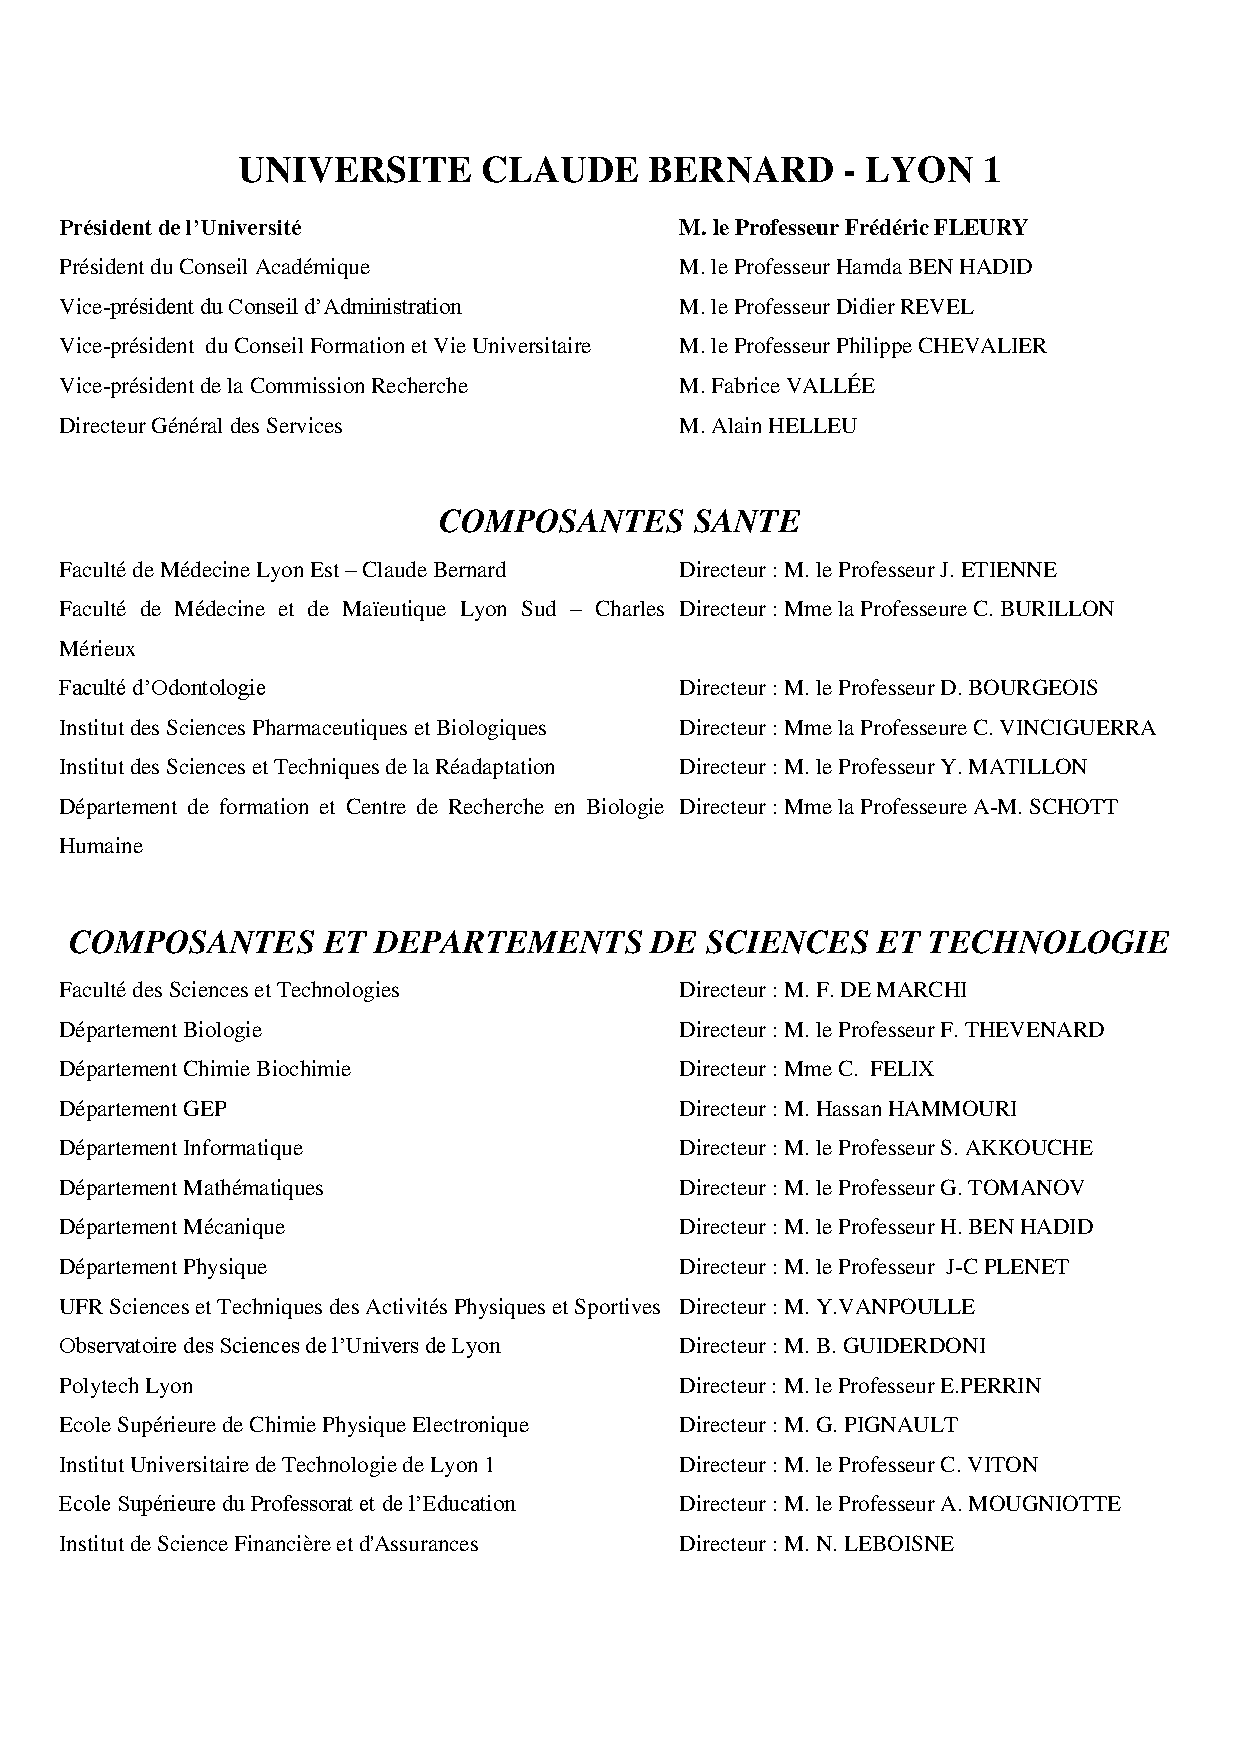
\includepdf[pages=-, fitpaper=true]{content/composante_lyon1.pdf}
